\documentclass{article}
\usepackage{graphicx,float}
\usepackage{amsmath,latexsym,amsfonts,amssymb,amsthm}

\usepackage[utf8]{inputenc}
\usepackage[english]{babel}
\usepackage[letterpaper,top=2cm,bottom=2cm,left=3cm,right=3cm,marginparwidth=1.75cm]{geometry}
\renewcommand{\baselinestretch}{1.667}


\title{Optimization Without Restrictions - Lab 2}
\author{Joris Plaščinskas}
\date{\today}


\begin{document}


    \maketitle
    \section*{Introduction \& Results}
        The goal of this laboratory work was to get familiar with optimization methods without restrictions. In this lab I implemented three methods: gradient descent, steepest descent, deform-able simplex search. The objective was to find the ratio of plots that gives the highest volume. The objective function for this task is negative squared volume: $-V^2 = p_1 \times p_2 \times p_3 \times -1$. After making a requirement for the sum of plots to be equal to one, we can derive one plot from the other two, that means that this function is now dependent on two parameters. Since the objective function is very simple and only has one local (and global) minima the results are highly dependent on the parameters. With my parameters, I got the best results using steepest descent method. After just 10 iterations the value was already $0.3333337$. Gradient descent after 10 iterations reached a plot 0 value of: $0.281536$. And simplex after 10 iterations: $0.317148$.
        \begin{figure}[H]
            \centering
            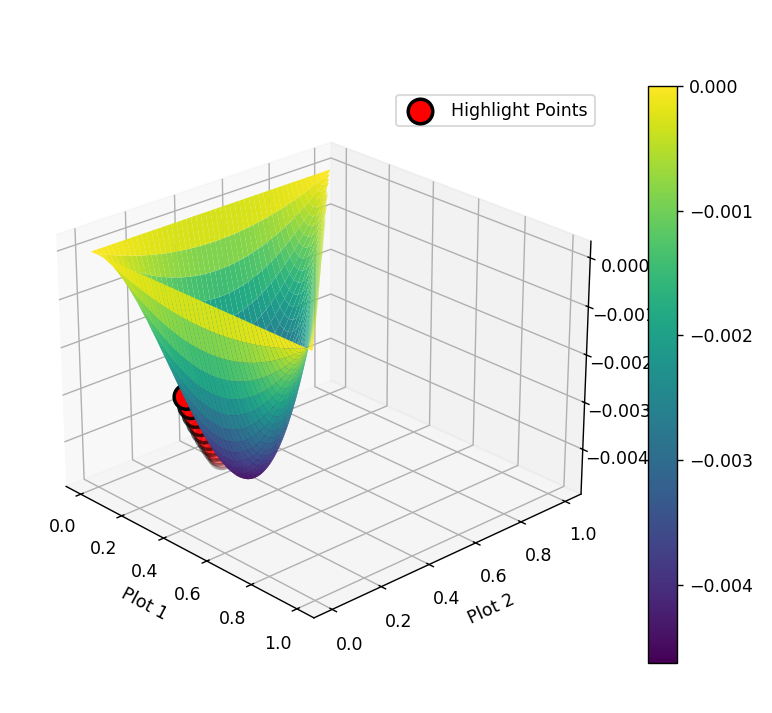
\includegraphics[width=0.5\textwidth]{gradient-02.png}
            \caption{Gradient Descent (0.2, 0.2)}
        \end{figure}
        \begin{figure}[H]
            \centering
            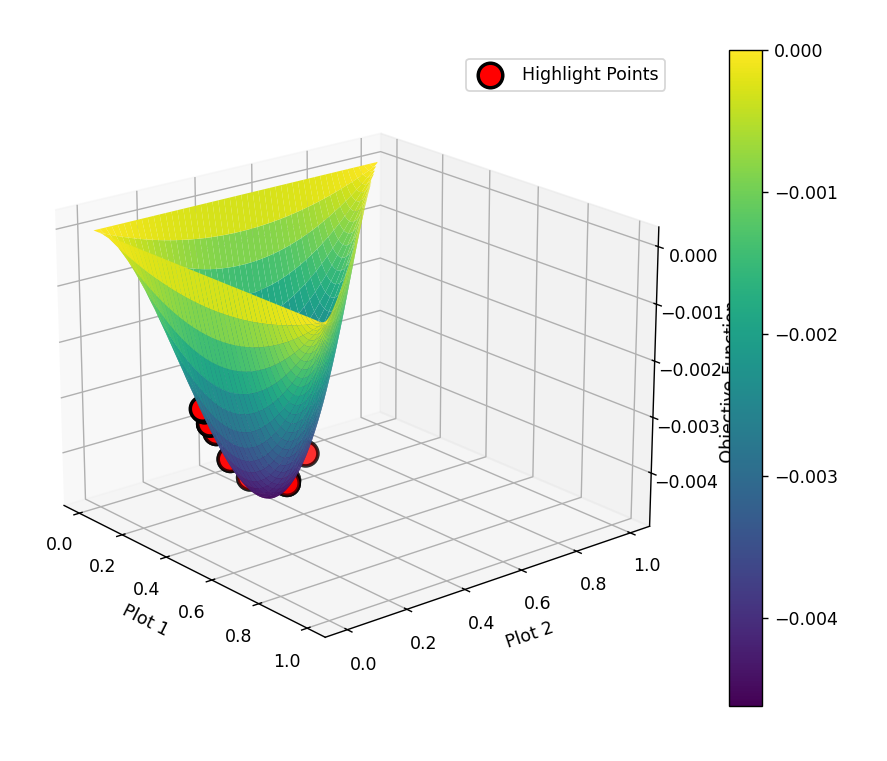
\includegraphics[width=0.5\textwidth]{simplex-02.png}
            \caption{Steepest Descent (0.2, 0.2)}
        \end{figure}
        \begin{figure}[H]
            \centering
            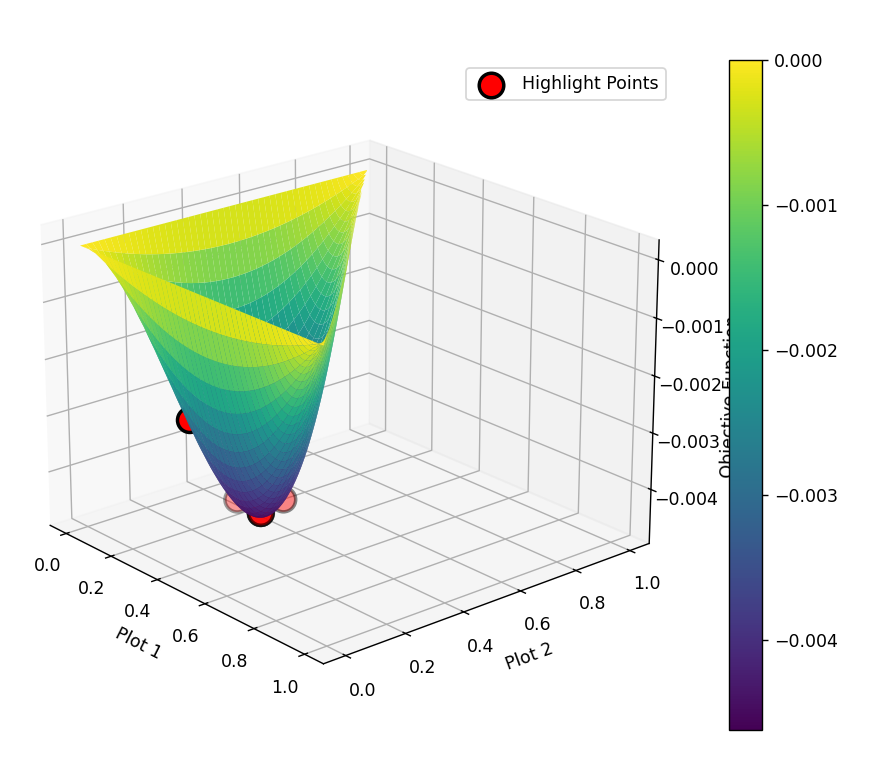
\includegraphics[width=0.5\textwidth]{steepest-02.png}
            \caption{Simplex Search (0.2, 0.2)}
        \end{figure}
        Other results are inside the code files.

    
\end{document}